\documentclass[11pt, oneside]{article}   	% use "amsart" instead of "article" for AMSLaTeX format
\usepackage{geometry}                		% See geometry.pdf to learn the layout options. There are lots.
\usepackage{textcomp}
\usepackage{hyperref}  % TODO: see page 94 of latex book
\geometry{letterpaper}                   		% ... or a4paper or a5paper or ... 
%\usepackage[parfill]{parskip}    		% Activate to begin paragraphs with an empty line rather than an indent
\usepackage{graphicx}				% Use pdf, png, jpg, or eps§ with pdflatex; use eps in DVI mode
								% TeX will automatically convert eps --> pdf in pdflatex		
\usepackage{amssymb}
\usepackage{amsmath}
\usepackage{relsize}

\title{CS181 / CSCI E-181 Spring 2014 Practical 3 \\ 
{\large Kaggle Team "Capt. Jinglehiemer"}
}
\author{
  David Wihl\\
  \texttt{davidwihl@gmail.com}
  \and
  Zachary Hendlin\\
  \texttt{zgh@mit.edu} 
}
%\date{}							% Activate to display a given date or no date

\begin{document}
\maketitle
\section*{Warm-Up}

We consider two approaches for classifying fruits (with length and width measurements provided) into one of three categories.

It is important to note that the data here is not perfectly linearly separable, as can be seen in the plot below:

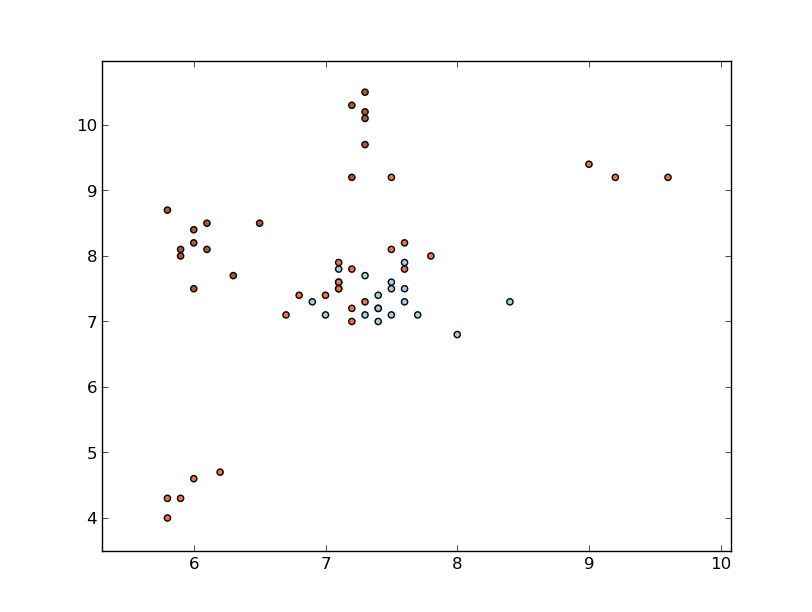
\includegraphics[scale=.6]{figure_3}

So the challenge becomes how we can best define mutually exclusive regions of the graph.

\subsection*{Logistic Classification}

Multiclass logistic classification seeks to define the weights that minimize:
\\
 $E(w_1, w_2, ..., w_K) =  -\sum\limits_{n=1}^N \sum\limits_{k=1}^K = t_{nk} ln_{nk}$ , 
as given in equation 4.108 in Bishop.
\
\\
Here our $w$ vector will have be $k x 3$ as we have a variable for height, weight, and then an offset term $w_0$.
\
\\
Since $k=3$, we fit 9 weights so as to minimize the error function. We use the Broyden Fletcher Goldfarb Shanno algorithm (BFGS) as implemented in the Scipy package. We select this because it provides a better approximation to the Hessian at each step.
\
\\
The error function achieves its minimum at 34.769598, and takes 44 iterations to converge.
\\
Once we have the weights:

\[
w=
  \begin{bmatrix}
    -7.35269067 & 2.48983592 & -1.17947522\\
    -3.65199071 & 1.66456348 & -0.81582258\\
    14.00478476 & -4.15564072 & 1.99410538\\	
	
  \end{bmatrix}
\]
\\
\
 we then use in the softmax function:
\
$y_k(\phi) = exp(a_k)/\sum\limits_{j=1}^K exp(a_j)$
\\
where $a$ is simply the dot product of $x$ and $w$,to evaluate which class has the highest likelihood for a particular data point. The point is then assigned to the class which has the highest class-conditional density.
\\
We get the resulting classification.
\begin{center}
  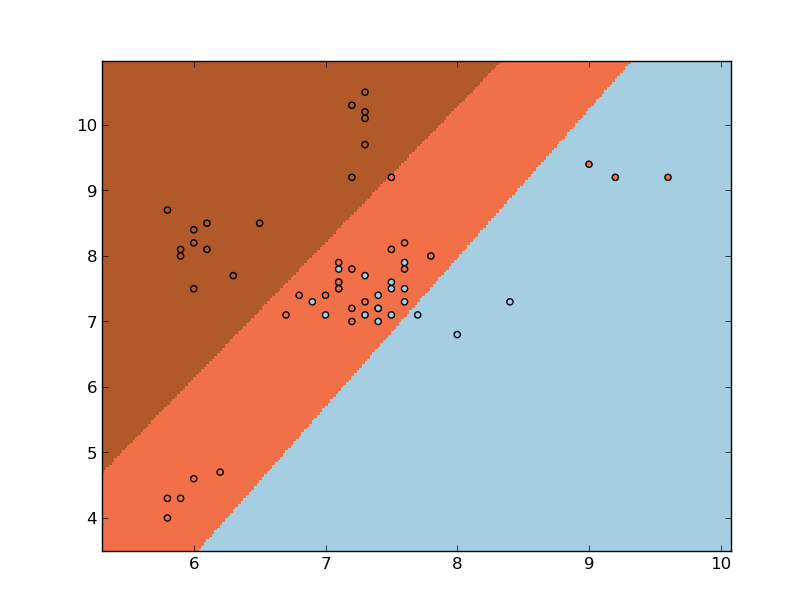
\includegraphics[scale=.55]{logistic_classifer}
\end{center}


\subsection*{Generative Model Classification}

Generative models attempt to determine, for each class $k$, a likelihood that a data point is generated by that particular class.
\\
\ We first calculate the prior likelihoods for each class $P(c_k)$
\\
\ And then recognizing we want $p(C_k |x_n)$ by applying Bayes rule, we need: $p(x_n |C_k)$.
\\
The multivariate normal is given by:
\
\\
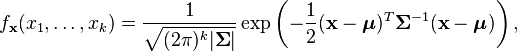
\includegraphics[scale=.5]{formula}
\
\\
where k=2 in our case because we have (1) height and (2) width.
\
\\
This gives us a probability density function for each class. We then apply Bayes rule:

$p(C_k |x_n) = p(x_n |C_k)  p(C_k) / \sum\limits_{j=1}^K p(x_n | c_j) * p(c_j)$

and note that we can ignore the denominator since it is the same for all classes.

We then have an assignment for each point to the highest likelihood class as shown in plot below.


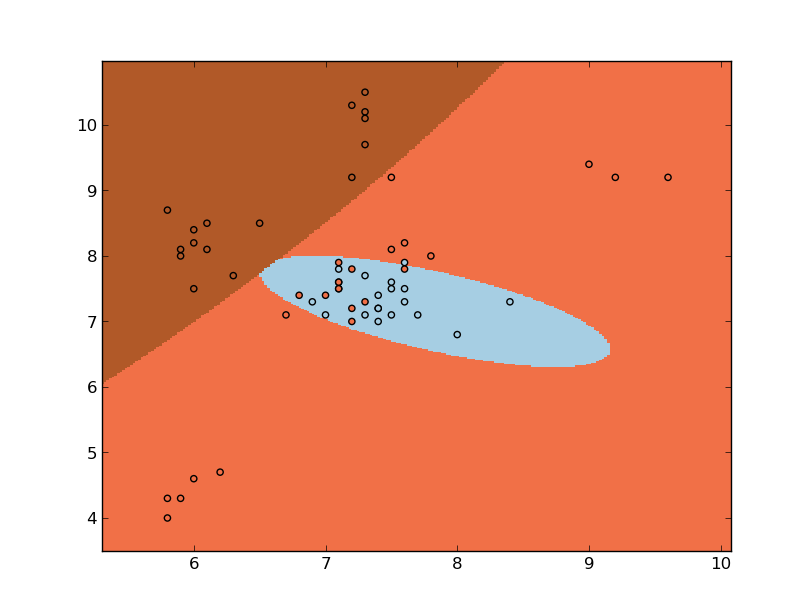
\includegraphics[scale=.6]{generative_classifier}


\subsection*{Warmup Summary}

As we can see from the graphs in the previos sections, allowing a non-linear decision boundry (as we did when we used the generative classifier) allowed more flexibility to capture clusters of points and indeed was more accurate at capturing the variation observed in the data.

\section*{Classifying Malicious Software}

\subsection*{Preliminary Data Analysis}

This problem was significantly more complex than the previous practicals due to a number of factors: unbalanced distribution of the targets, sparsity of the data, conversion of hierarchical XML data into rectangular matrices, hashing of non-numeric values and unclear value of certain attributes in the data. 

Significant experimentation was required to iterate over feature engineering, classifier choice, permutations of ensembles of classifiers and hyper parameter optimization.

The first step was a significant refactoring of the sample code in order to separate vectorization, classification, validation and submission.

\subsection*{Using Cross-validation}

Very early we created a test harness that enabled testing of $n$ iterations (default 5) over cross-validation sets consisting of 30\%, 20\% and 10\% of the data. This proved very valuable as we experimented. In total, we ran over 200 cross-validation tests each consisting of 15 different passes.

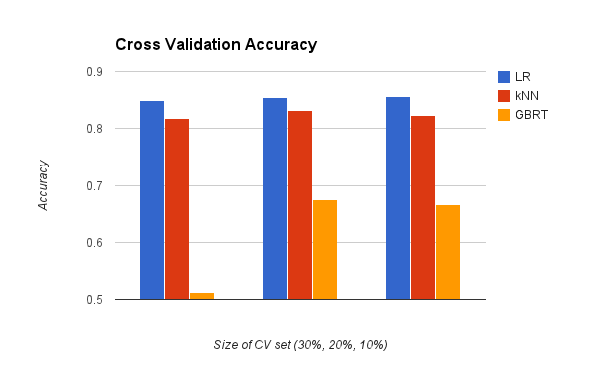
\includegraphics[scale=.6]{cv_error}


\subsection*{Per File Feature Engineering}

The first vectorizer took simple counts of each different type of system call as well as per-process (e.g. `startreason', `terminationreason', `username', `executionstatus', `applicationtype') and per-file metrics coupled with an unoptimized logistic regression. This enabled us to achieve a 75\% accuracy on our second Kaggle submission.

\subsection*{Comparing Classifiers and Tuning Hyperparameters}

We attempted a number of different classifiers (Logistic Regression, SVM, kNearest Neighbor, Gradient Boosting). Logistic Regression provided the most consistently accurate predictions. kNearest Neighbor provided very accurate results only when the prediction probability estimate was high. This combination proved useful when combining classifiers later on.

\subsection*{Pruning the Dimensions}

We took two complementary approaches to prune the dimensions.
\begin{enumerate}
  \item We examined the weights of each of the classifiers to see which dimensions were not producing a signal. Using the mean and standard deviation of the resulting matrix, we noted any features where abs(mean) $<$ 0.001 and std $< $0.01.
  \item We exported our Design Matrix to a CSV and then used tools in R to run a linear regression and see the predicted values of the coefficients. 
\end{enumerate}

We then pruned back approximately 35 features that provided no value (and ran cross validation to recheck).

In doing this, we found that the process file's MD5 hash directly correlated to at least one virus definition. This is unsurprising given that MD5 is a quick and effective means to determine if a file has been tampered with.

We actually found that combining two different sets of classifers worked under different situations. For instance, we found that the summary features had the most overall explanatory power, but that more specific information on each process was useful in specifically identifying certain cases.

Interestingly, we found that the hyper-detailed information on each process feature was actually less useful on average than more aggregated features. This points to the importance of feature engineering and trying to capture key elements of the underlying data rather than simply adding features without as much thought to why they might make sense and if they are the best representation of key attributes.

\subsection*{Per Thread Feature Engineering}

We attempted a second, separate model of per system-call metrics, consisting of features such as `successful', `protect', `user', `target' attributes. Attributes of type string that had potential value were hashed into a numeric form. This resulted in a design matrix of over 13000000 rows $\times$ 14 features.

While the initial results were promising on a subset of the training data, this resulted in exhausting capacity on 16 Gb machines even when using sparse matrices.

\subsection*{Combining Classifiers}

We examined several options for combining the classifiers, including bagging, boosting and Committees. As Bishop points out ``these simple mixtures extend the flexibility of linear models to include more complex predictive distributions, they are still very limited." (pg 672).

We attempted a novel approach to combining classifiers. Each of the linear multi-class classifiers we used provided for each prediction a probability of the sample in each of the classes.\cite{sklearn}. Through several test runs, we measured each classifier's $max(class\_probability)$ to accuracy. We found the threshold value for $<$1\% error rate for each classifier across the cross validation sets. 

\begin{figure}[h!] 
  \centering
  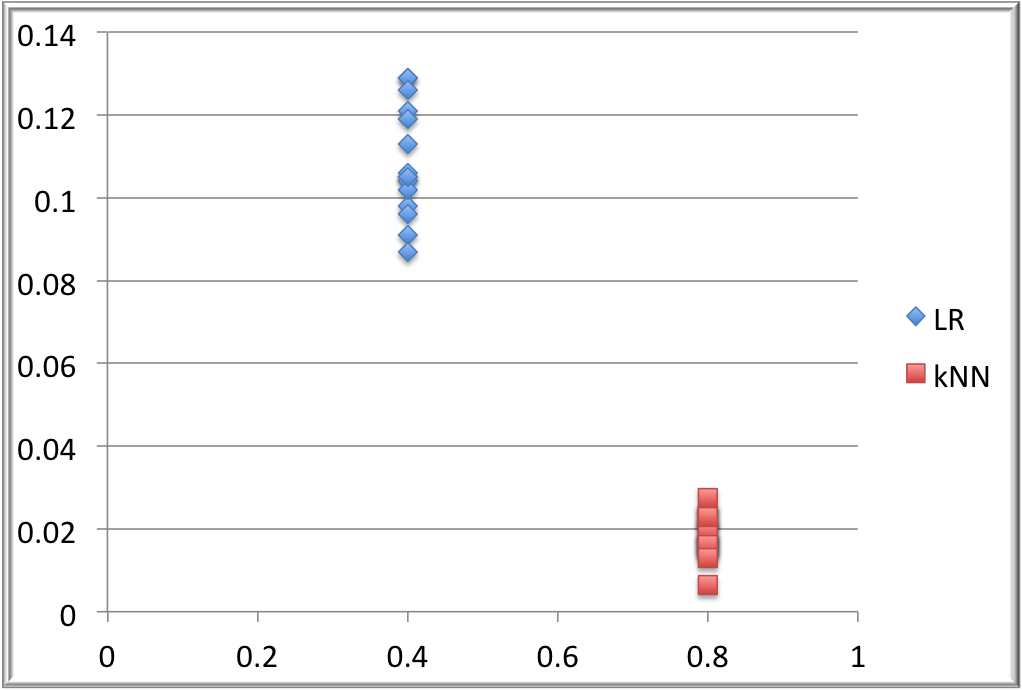
\includegraphics[scale=0.5]{accuracy}
  \caption{Predicted Probability Threshold vs. Error Rate}
\end{figure}


During prediction, if the classifier's probability was higher than this threshold, it was given the vote. If one classifier had a significantly higher confidence level (determined empirically to be 0.4), it was given the vote. If no classifier had a high confidence, it was given to Logistic Regression as it had the lowest overall error rate. After implementation, we found that Alpaydin refers to this technique as \emph{Dynamic Classifier Selection}.\cite{alpaydin}



During our cross-validation runs, this technique increased our accuracy by approximately 3\%. However, our Kaggle score did not change commensurately, likely due to overfitting in spite of our cross validation. 


\subsection*{Quality Check prior to Submission}

After a couple of poor submissions due to bugs in our implementation, we created a sanity check for submissions. This would be useful in real world scenarios to ensure that the predictions are within a reasonable tolerance prior to putting new models into production. The sanity check displayed a distribution of classes to ensure that no unusual skews were occurring. We did not presume that a subsequent day would have the same distribution of viruses as the training set. However once Kaggle informed us that we were 75\% accurate on the public leader board, we wanted to at least ensure that we weren't wasting any further Kaggle submissions. 

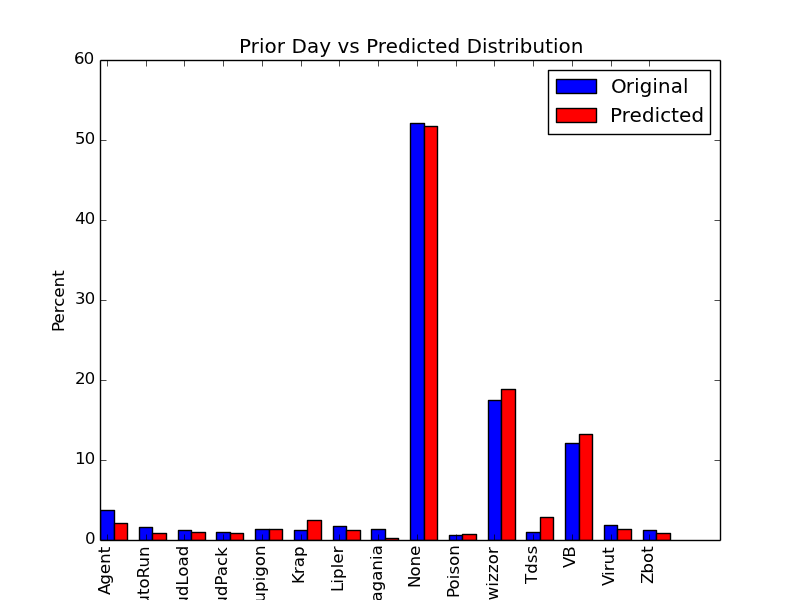
\includegraphics[scale=.65]{predictVactual}

\subsection*{Exotic Classifiers}

We examined and did preliminary experiments with two different approaches: Exemplar SVM \cite{exemplar}  and Theano / Deep Learning \cite{deep}. While the reading was interesting, in both cases, the quality of the code and library precluded us from pursuing these options in the time available. We hit a bug in Theano when using the Scipy Sparse array. We intend to continue exploring Theano outside the scope of this exercise.


\section*{Conclusion}

We conclude from this practical that considering what classifiers work well over what ranges is extremely important. That is, when we combined models to allow them to effectively apply over different 'ranges' of the data, we were able to capture more nuanced effects than if we had simply attempted a single set of classifers that was applied to all data across the range. 

This idea -- which is also true in decision trees and random forests -- effectively allows the function mapping the data to be more specific to the variability observed in the data and points to an important idea for us to consider in future machine learning projects.

This was a valuable exercise in understanding the state of the art in multi-class classification with real-world, sparse hierarchical data. Given the preponderance of business data that exists in relational schemas including master-detail, it was enlightening to see how much room there is for exploration in this area.

The permutations of features, classifiers and hyper parameters grow geometrically without many significant tools to provide automated means of attacking the problem. This is an area we would be interested in pursuing with further research.

\begin{thebibliography}{1}

 \bibitem{sklearn} Classifier comparison:
  http://scikit-learn.org/stable/auto\_examples/plot\_classifier\_comparison.html
  
  \bibitem{alpaydin} Alpaydin, Ethem, \emph{Machine Learning}, ISBN 978-026201243-0

 \bibitem{exemplar} Tomasz Malisiewicz and Abhinav Gupta and Alexei A. Efros, \emph{Ensemble of Exemplar-SVMs for Object Detection and Beyond} ICCV 2011

 \bibitem{deep} Bengio, Yoshua, \emph{Learning deep architectures for $\{AI\}$}, Now Publishers, 2009

  \end{thebibliography}

\end{document}  
